% !TEX root = /workplace/presa2/main.tex

\documentclass[aspectratio=169]{beamer}
\usepackage{import}

\import{preamble/}{packages.tex}
\import{preamble/}{base.tex}
\import{preamble/}{plot_settings.tex}

\title[ECC]{Популярно о криптографии на \\[0.5em] эллиптических кривых}
\author[RNDSOFT]{ltv1304@yandex.ru}
\institute[]{RNDSOFT}
\date[]{\today}

\begin{document}
  
  \setbeamercolor{background canvas}{bg=RNDSgreen} 
  \begin{frame}[plain]
    \centering
    \hspace*{-2cm}
    \begin{minipage}{\dimexpr\textwidth+2cm\relax}
      \centering
      \titlepage
    \end{minipage}
  \end{frame}

  \setbeamercolor{background canvas}{bg=black} 
  \begin{frame}[plain]
    \centering
    \hspace*{-2cm}
    \begin{minipage}{\dimexpr\textwidth+2cm\relax}
      \centering
      {\usebeamerfont{title}\textcolor{red}{\uppercase{дислеймер}}\par}
      
      \bigskip
      \textcolor{white}{
        Этот доклад родился как ответы на мои же вопросы при попытке разобраться в некоторых вопросах асимметричной криптографии. 
        Доклад не претендует на научную верность или академическую точность, рассказываю как сам понял. 
        \textcolor{red}{\uppercase{внимание!}} текст подготовлен с использованием ИИ, имейте это ввиду!!!
      }
    \end{minipage}
  \end{frame}


  \setbeamercolor{background canvas}{bg=white}
  \section{Введение}
    \begin{frame}
  \begin{center}
    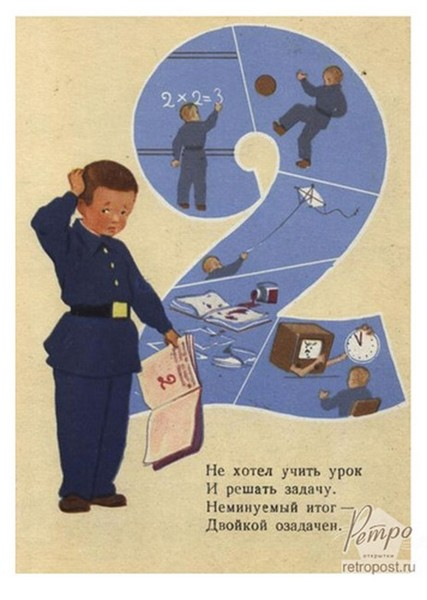
\includegraphics[height=0.9\textheight]{static/img/slacker.jpg}
  \end{center}
\end{frame}

    \subsection{Конечные поля}
      \begin{frame}
        Применение конечных полей:
        \begin{itemize}[label=---]  
          \item криптография: ECC, AES, хеширование;
          \item телекоммуникации: алгоритмы помехоустойчивого кодирования, быстрые алгоритмы свертки и фильтрации, FFT;
          \item IT: ГПСЧ, алгоритмы хеширования, блокчейн, распределенные СУБД, алгоритмы сжатия.
        \end{itemize}
      \end{frame}
    \subsection{Историческая справка}
      \subsubsection{Алгебраические уравнения}
          \begin{frame}
    \begin{center}
       \onslide<1-> {
            \[ ax^n+bx^{n-1}+...+px^2+qx+r = 0 \]
       } 
       \onslide<2->{
       \begin{itemize}
        \item {
            Древний мир (до V века н.э.)
            \[ ax+b = 0; ax^2+bx+c = 0 \]
            }
        \item{
            Средневековье и исламский мир (V–XV века)
            \[ ax^3+bx^2+cx+e = 0 \]
        } 
        \item {
            Эпоха Возрождения (XVI век)
            \[ ax^4 + bx^3+cx^2+ex+f = 0 \]
        }
        \item {
            Новое время (XVII–XIX века)
            \[ ax^5+bx+c = 0 \]
        }
        \item Современная эпоха (XX–XXI века)
       \end{itemize}
       }
    \end{center}
\end{frame}

      \subsubsection{Эварист Галуа}
          \begin{frame}
  \begin{center}
    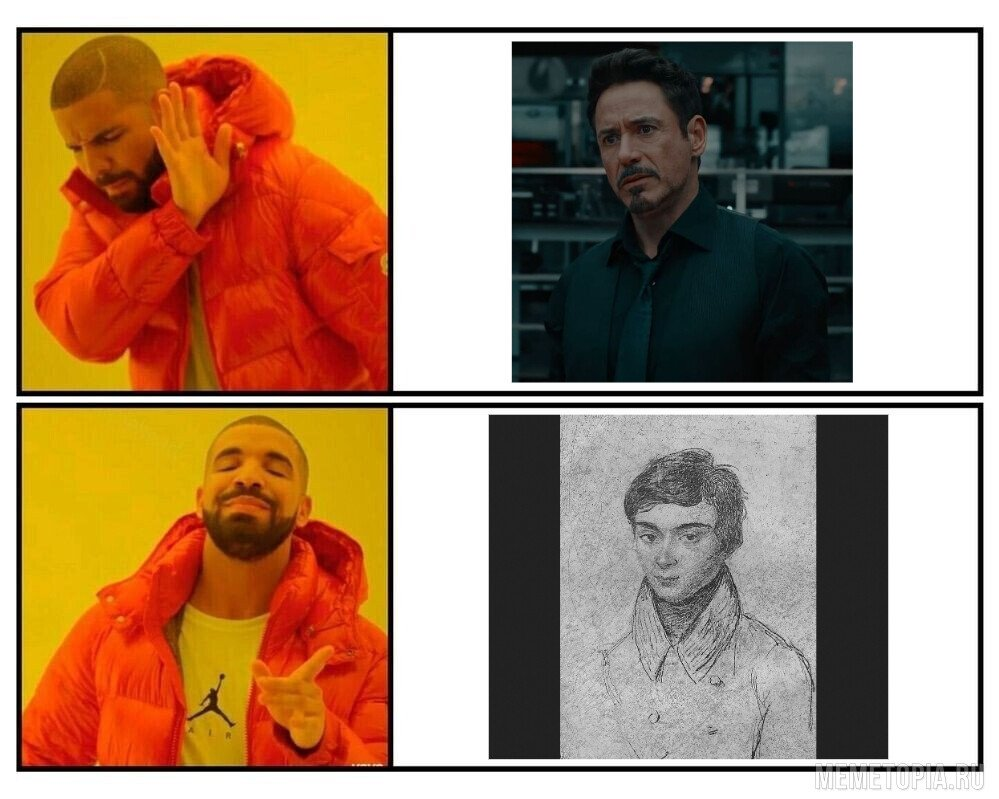
\includegraphics[height=0.9\textheight]{static/img/mem.jpeg}
  \end{center}
\end{frame}

  \section{Основная часть}
    \subsection{Конечные поля}
      \subsubsection{Определение}
        \begin{frame}
  \[ y^2 = x^3+ax+b - \text{эллиптическая кривая} \]
  \[ x^2/a^2+y^2/b^2 = 1 - \text{эллипс} \]
  \centering  
  \begin{tikzpicture}
    \begin{axis}[
      width=5cm, % Ширина графика
      height=6cm, % Высота графика
      domain=-5:5, % Диапазон по оси X
      y domain=-5:5, % Диапазон по оси Y
      samples=50, % Количество точек для построения
      smooth, % Сглаживание графика
      grid=both, % Включаем сетку
      enlargelimits=true, % Расширяем границы графика
      view={0}{90}, % Вид сверху (2D)
      name=plot1 % Имя для первого графика
  ]
  \addplot3[
    contour gnuplot={
        levels={0},
        labels=false,
        draw color=RNDSblue,
        cmd={
          gnuplot -c ./graphs/elliptic_curve.gp "./tmp/main_contourtmp0.table"
        }
    },
    thick,
    RNDSblue,
    domain=-3:4,
    y domain=-9:9
] {y^2 - x^3 - 9};
 \legend{secp256k1} % Легенда
\end{axis}
  
    % Второй график: повёрнутый эллипс
    \begin{axis}[
      width=5cm, % Ширина графика
      height=6cm, % Высота графика
      domain=-5:5, % Диапазон по оси X
      y domain=-5:5, % Диапазон по оси Y
      samples=50, % Количество точек для построения
      smooth, % Сглаживание графика
      grid=both, % Включаем сетку
      enlargelimits=true, % Расширяем границы графика
      view={0}{90}, % Вид сверху (2D)
      at={(plot1.right of north east)}, % Позиция второго графика
      anchor=left of north west % Привязка
    ]
      % Рисуем повёрнутый эллипс
      \addplot[
        red,
        thick,
        domain=0:360,
        samples=100,
        variable=\t,
      ] ({cos(45) * 2*cos(t) + sin(45) * sin(t)}, {-sin(45) * 2*cos(t) + cos(45) * sin(t)});
      \legend{Это эллипс} % Легенда
    \end{axis}
  \end{tikzpicture}
  \end{frame}
        \begin{frame}
    \onslide<1->{
        \begin{tcolorbox}[colback=RNDSblue!5!white,colframe=RNDSblue!75!black,title=Операция сложения в конечном поле $P_{5}$ ]
            \[ a +_{f} b = (a+b) \% P;\quad 3 + 4 = 7 \% 5 = 2 \]
        \end{tcolorbox}
    
        \begin{tcolorbox}[colback=RNDSblue!5!white,colframe=RNDSblue!75!black,title=Операция умножения в конечном поле $P_{5}$]
            \[ a \times_{f} b = (a*b) \% P;\quad 3 * 3 = 9 \% 5 = 4 \]
        \end{tcolorbox}
    
        \begin{tcolorbox}[colback=RNDSblue!5!white,colframe=RNDSblue!75!black,title=Операция деления в конечном поле $P_{5}$]
            \[ a /_{f} b = a * b^{P-2} \% P;\quad 4 / 3 = 4*3^{5-2} \% 5 = 3 \]
        \end{tcolorbox}
    
        \begin{tcolorbox}[colback=RNDSblue!5!white,colframe=RNDSblue!75!black,title=Операция вычитания в конечном поле $P_{5}$]
            \[ a -_{f} b = (a - b) \% P;\quad 2 - 4 \only<2->{= -2 \% 5 = 3} \]
        \end{tcolorbox}
    }
\end{frame}
        \begin{frame}
    \begin{tcolorbox}[colback=RNDSyelow!5!white,colframe=RNDSyelow!75!black,title=Нулевой элемент множества ]
        \[ A + Z = A \]
    \end{tcolorbox}

    \begin{tcolorbox}[colback=RNDSyelow!5!white,colframe=RNDSyelow!75!black,title=Единичный элемент множества ]
        \[ A \times I = A \]
    \end{tcolorbox}

    \begin{tcolorbox}[colback=RNDSyelow!5!white,colframe=RNDSyelow!75!black,title=Отрицательный элемент ]
        \[ A + (-A) = 0 \]
    \end{tcolorbox}

    \begin{tcolorbox}[colback=RNDSyelow!5!white,colframe=RNDSyelow!75!black,title=Обратный элемент множества ]
        \[ A \times A^{-1} = A \]
    \end{tcolorbox}
\end{frame}
      \subsubsection{Зачем они нужны}
        \begin{frame}
\begin{enumerate}[label={\alph*)}]
    \item Конечность и управляемость
    \item Арифметика по модулю и обратимость
    \item Защита от атак перебором
    \item Эффективность вычислений
\end{enumerate}
\end{frame}
    \subsection{Эллиптические кривые}
      \subsubsection{Определение}
        \begin{frame}
  \[ y^2 = x^3+ax+b - \text{эллиптическая кривая} \]
  \[ x^2/a^2+y^2/b^2 = 1 - \text{эллипс} \]
  \centering  
  \begin{tikzpicture}
    \begin{axis}[
      width=5cm, % Ширина графика
      height=6cm, % Высота графика
      domain=-5:5, % Диапазон по оси X
      y domain=-5:5, % Диапазон по оси Y
      samples=50, % Количество точек для построения
      smooth, % Сглаживание графика
      grid=both, % Включаем сетку
      enlargelimits=true, % Расширяем границы графика
      view={0}{90}, % Вид сверху (2D)
      name=plot1 % Имя для первого графика
  ]
  \addplot3[
    contour gnuplot={
        levels={0},
        labels=false,
        draw color=RNDSblue,
        cmd={
          gnuplot -c ./graphs/elliptic_curve.gp "./tmp/main_contourtmp0.table"
        }
    },
    thick,
    RNDSblue,
    domain=-3:4,
    y domain=-9:9
] {y^2 - x^3 - 9};
 \legend{secp256k1} % Легенда
\end{axis}
  
    % Второй график: повёрнутый эллипс
    \begin{axis}[
      width=5cm, % Ширина графика
      height=6cm, % Высота графика
      domain=-5:5, % Диапазон по оси X
      y domain=-5:5, % Диапазон по оси Y
      samples=50, % Количество точек для построения
      smooth, % Сглаживание графика
      grid=both, % Включаем сетку
      enlargelimits=true, % Расширяем границы графика
      view={0}{90}, % Вид сверху (2D)
      at={(plot1.right of north east)}, % Позиция второго графика
      anchor=left of north west % Привязка
    ]
      % Рисуем повёрнутый эллипс
      \addplot[
        red,
        thick,
        domain=0:360,
        samples=100,
        variable=\t,
      ] ({cos(45) * 2*cos(t) + sin(45) * sin(t)}, {-sin(45) * 2*cos(t) + cos(45) * sin(t)});
      \legend{Это эллипс} % Легенда
    \end{axis}
  \end{tikzpicture}
  \end{frame}
      \subsubsection{Арифметика точек}
        \begin{frame}
  \begin{columns}[T]
    \hspace{-1.5cm}\begin{column}{0.7\textwidth}
      \begin{tikzpicture}
        \begin{axis}[
          my axis style,
          xmin=-3, xmax=4,
          ymin=-9, ymax=9,
          zmin=-1, zmax=1,
          view={0}{90},
        ]
          \addplot3[
            contour gnuplot={
              levels={0},
              labels=false,
              draw color=RNDSblue,
              cmd={
                gnuplot -c ./graphs/elliptic_curve.gp "./tmp/main_contourtmp1.table"
              }
            },
            thick,
            RNDSblue,
            domain=-3:4,
            y domain=-9:9
          ] {y^2 - x^3 - 9};
          \addplot[RNDSgreen, thick, domain=-3:4] {x + 3}; 
          \addplot[dashed, ultra thick, RNDSgreen, no marks] coordinates {(0, 3) (0, -3)};
          \node[label={180:{$A$}}, circle, draw, thick, color=RNDSgreen, fill=white, inner sep=2pt] at (axis cs:-2, 1) {};
          \node[label={180:{$B$}}, circle, draw, thick, color=RNDSgreen, fill=white, inner sep=2pt] at (axis cs:3, 6) {};
          \node[label={[yshift=0.5em]180:{$C'$}}, circle, draw, thick, color=RNDSgreen, fill=RNDSgreen, inner sep=2pt] at (axis cs:0, 3) {};
          \node[label={[yshift=0.5em]180:{$C$}}, circle, draw, thick, color=RNDSgreen, fill=RNDSgreen, inner sep=2pt] at (axis cs:0, -3) {};
        \end{axis}
      \end{tikzpicture}
    \end{column}
    \hspace{-2.5cm}\begin{column}{0.3\textwidth}
      \begin{enumerate}[label=\alph*),nosep ]
        \item $ A + I = A $
        \item $ A + (-A) = I $
        \item $A + B = B + A$
        \item $ (A + B) + C = A + (B + C) $
      \end{enumerate}
    \end{column}
  \end{columns}
\end{frame}
        \begin{frame}
  \centering
  \begin{tikzpicture}
    \begin{axis}[
      my axis style,
      xmin=-3, xmax=4,
      ymin=-9, ymax=9,
      zmin=-1, zmax=1,
      view={0}{90},
      width=0.8\textwidth,
    ]
      \addplot3[
        contour gnuplot={
          levels={0},
          labels=false,
          draw color=RNDSblue,
          cmd={
            gnuplot -c ./graphs/elliptic_curve.gp "./tmp/main_contourtmp3.table"
          }
        },
        thick,
        blue,
        domain=-3:4,
        y domain=-9:9
      ] {y^2 - x^3 - 9};
    
      \draw[RNDSgreen, ultra thick] 
        (axis cs:1,\pgfkeysvalueof{/pgfplots/ymin}) -- 
        (axis cs:1,\pgfkeysvalueof{/pgfplots/ymax});
      \node[label={[yshift=0.5em]180:{$A$}}, circle, draw, thick, color=RNDSgreen, fill=RNDSgreen, inner sep=2pt] at (axis cs:1, 3.1603) {};
      \node[label={[yshift=0.5em]180:{$A'$}}, circle, draw, thick, color=RNDSgreen, fill=RNDSgreen, inner sep=2pt] at (axis cs:1, -3.1603) {};
    \end{axis}
  \end{tikzpicture}
\end{frame}
        \begin{frame}
  \centering
  \begin{tikzpicture}
    \begin{axis}[
      my axis style,
      xmin=-3, xmax=4,
      ymin=-9, ymax=9,
      zmin=-1, zmax=1,
      view={0}{90},
      width=0.8\textwidth
    ]
      \addplot3[
        contour gnuplot={
          levels={0},
          labels=false,
          draw color=RNDSblue,
          cmd={
            gnuplot -c ./graphs/elliptic_curve.gp "./tmp/main_contourtmp2.table"
          }
        },
        thick,
        RNDSblue,
        domain=-3:4,
        y domain=-9:9
      ] {y^2 - x^3 - 9};

      \addplot[domain=-3:4, RNDSgreen, ultra thick] {0.948*x + 3.835};
      \node[label={[yshift=0.5em]180:{$C$}}, circle, draw, thick, color=RNDSgreen, fill=RNDSgreen, inner sep=2pt] at (axis cs:-1.28571,2.61589) {};
    \end{axis}
  \end{tikzpicture}
\end{frame}
    \subsection{Скрещиваем}
      \subsubsection{Определение}
        \begin{frame}
  \begin{tikzpicture}
    \begin{axis}[
      my axis style,
      xmin=0, xmax=103,
      ymin=0, ymax=103,
      at={((0, -2em))},
      anchor=north west,
    ]
        \addplot[my point style] table {./graphs/line_ander_field.dat};
    \end{axis}
  \end{tikzpicture}
\end{frame}
        \begin{frame}
  \begin{tikzpicture}
    \begin{axis}[
      my axis style,
      xmin=0, xmax=103,
      ymin=0, ymax=103,
      at={((0, -2em))},
      anchor=north west,
    ]
        \addplot[my point style] table {./graphs/curve_ander_field.dat};
    \end{axis}
  \end{tikzpicture}
\end{frame}
      \subsubsection{Скалярное умножение}
        \begin{frame}
  \begin{columns}[T]
    \hspace{-1.5cm}\begin{column}{0.7\textwidth}
      \begin{tikzpicture}
        \begin{axis}[
          my axis style,
          xmin=-3, xmax=4,
          ymin=-9, ymax=9,
          zmin=-1, zmax=1,
          view={0}{90},
        ]
          \addplot3[
            contour gnuplot={
              levels={0},
              labels=false,
              draw color=RNDSblue,
              cmd={
                gnuplot -c ./graphs/elliptic_curve.gp "./tmp/main_contourtmp4.table"
              }
            },
            thick,
            blue,
            domain=-3:4,
            y domain=-9:9
          ] {y^2 - x^3 - 9};
          \node[label={[yshift=0.5em]180:{$G$}}, circle, draw, thick, color=RNDSgreen, fill=RNDSgreen, inner sep=2pt] at (axis cs:-1.28571, 2.61589) {};
          \node[label={[yshift=0.5em]180:{$2G$}}, circle, draw, thick, color=RNDSgreen, fill=RNDSgreen, inner sep=2pt] at (axis cs:3.463, -7.118) {};
          \node[label={[yshift=0.5em]180:{$3G$}}, circle, draw, thick, color=RNDSgreen, fill=RNDSgreen, inner sep=2pt] at (axis cs:2, 4.11977) {};
          \addplot[dashed, ultra thick, RNDSgreen, no marks] coordinates {(3.463, 7.118) (3.463, -7.118)};
          \addplot[dashed, ultra thick, RNDSyelow, no marks] coordinates {(2, -4.11977) (2, 4.11977)};
          \addplot[domain=-3:4, RNDSgreen, ultra thick] {0.948*x + 3.835};
          \addplot[domain=-2:4, RNDSyelow, ultra thick] {-2.050*x - 0.020};
          \addplot[domain=-3:4, RNDSorange, thick] {0.4577*x + 3.2044};
        \end{axis}
      \end{tikzpicture}
    \end{column}
    \hspace{-2.5cm}\begin{column}{0.3\textwidth}
        $ \{ G, 2G, 3G, 4G, ..., nG \} $
    \end{column}
  \end{columns}
\end{frame}
        \begin{frame}
  \begin{columns}
  \begin{column}{0.8\textwidth}
      \centering
      \begin{tikzpicture}

\begin{axis}[
  my axis style,
  xmin=0, xmax=103,
  ymin=0, ymax=103,
]

\addplot[my faded_point style, skip coords between index={108}{115}] table {./graphs/curve_ander_field.dat};

\addplot[
  my point style,
  my point_label plot,
  point meta=explicit symbolic,  % Разрешаем метаданные для подписей
  nodes near coords=\pgfmathparse{int(\coordindex+2)}\pgfmathresult,
  ] table {./graphs/group.dat};

\node[label={[font=\bfseries, yshift=0.5em, text=RNDSblue]180:{G}}, circle, draw=RNDSblue, fill=RNDSblue, thick, inner sep=2pt, minimum size=2pt] at (axis cs:100, 17) {};

\end{axis}
\end{tikzpicture}
  \end{column}
  \begin{column}{0.3\textwidth}
      $G = (100,17)$
      \[
      \begin{array}{r|l}
          G2 & (78,55) \\
          G3 & (8,2) \\
          G4 & (59,2) \\
          G5 & (7,12) \\
          G6 & (22,47) \\
          G7 & (36,101) \\
          G8 & (85,47) \\
          G9 & (25,39) \\
          G10 & (38,17) \\
          G11 & (38,86) \\
          G12 & (17,39) \\
          *** & ***     \\
      G36 & (100,86) \\
      \end{array}
      \]
  \end{column}
\end{columns}
\end{frame}

    \subsection{Криптография}
      \subsubsection{Определение}
        \begin{frame}
  \onslide<1->{
    \begin{enumerate}[label={\alph*}]
      \item общий вид уравнения эллиптической кривой
        \begin{overlayarea}{\textwidth}{3em}
          \only<2->{\[ y^2 = x^3 + 7 \]}
        \end{overlayarea}
      \item порядок конечного поля (кол-во элементов)
        \begin{overlayarea}{\textwidth}{1em}
          \only<2->{\resizebox{0.9\linewidth}{!}{$ P = \text{0xFFFFFFFFFFFFFFFFFFFFFFFFFFFFFFFFFFFFFFFFFFFFFFFFFFFFFFFEFFFFFC2F}_{16} $}}
        \end{overlayarea}
      \item генераторная точка
        \begin{overlayarea}{\textwidth}{2em}
          \only<2->{
            \resizebox{0.9\linewidth}{!}{$G_x =   \text{0x79BE667EF9DCBBAC55A06295CE870B07029BFCDB2DCE28D959F2815B16F81798}_{16}$};
            \resizebox{0.9\linewidth}{!}{$G_y = \text{0x483ADA7726A3C4655DA4FBFC0E1108A8FD17B448A68554199C47D08FFB10D4B8}_{16}$};
          }
        \end{overlayarea}
      \item количество элементов в группе
        \begin{overlayarea}{\textwidth}{1em}
          \only<2->{
            \resizebox{0.9\linewidth}{!}{$ n = \text{0xFFFFFFFFFFFFFFFFFFFFFFFFFFFFFFFEBAAEDCE6AF48A03BBFD25E8CD0364141}_{16} $}
          }
        \end{overlayarea}
    \end{enumerate}
    }
\end{frame}
        \begin{frame}
  \begin{overlayarea}{\textwidth}{0.8\textheight}
    \[ G, 2G, 3G, 4G, ..., nG \]
    \[ Ge = P \]
    
    \vspace{1cm}
    
    \only<2->{
      где:
      \begin{itemize}
        \item $G$ - исходная точка группы
        \item $e$ - множитель
        \item $P$ - точка группы
      \end{itemize}
    }
    \only<3->{
      или:
      \begin{itemize}
        \item $G$ - исходная точка группы
        \item $e$ - закрытый ключ
        \item $P$ - открытый ключ
      \end{itemize}
    }
  \end{overlayarea}
\end{frame}
        \begin{frame}
    Чтобы осознать порядок величины $2^{256} \approx 10^{77}$:
    \begin{itemize}[label=*]
        \item количество атомов на планете Земля: $~ 10^{50}$;
        \item количество атомов в Солнечной системе: $~ 10^{57}$; 
        \item количество атомов в галактике Млечный путь: $~ 10^{68}$; 
        \item количество атомов во вселенной: $~ 10^{80}$.
    \end{itemize}

\end{frame}
      \subsubsection{Подписание и верификация}
        \begin{frame}
    Приемной стороне передается набор 256 битных чисел: 
      \begin{itemize}[label=---]  
        \item подпись;
        \item случайная величина;
        \item открытый ключ; 
        \item значение вычисленное из этих величин с применением закрытого ключа;
      \end{itemize}
  \end{frame}

  \section{Заключение}
    \subsection{Квантовый компьютер}
      \begin{frame}
  \begin{center}
    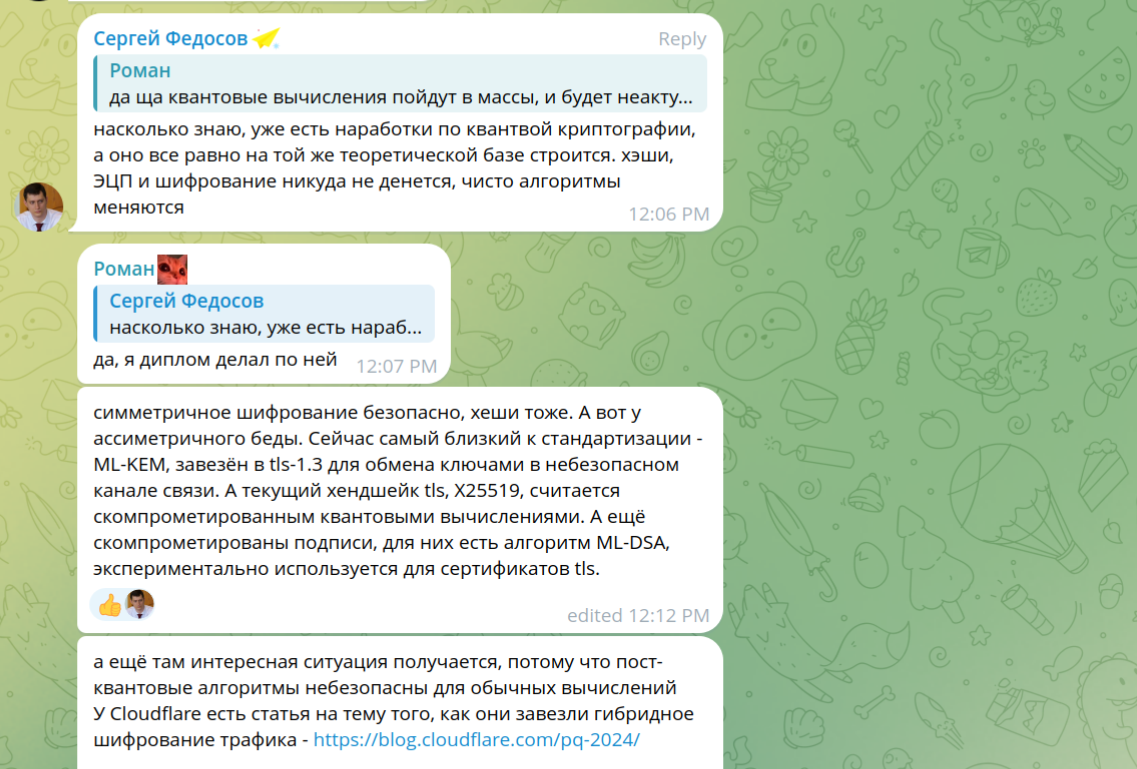
\includegraphics[width=0.8\textwidth]{static/img/chat.png}
  \end{center}
\end{frame}
    \subsection{АНБ}
      \begin{frame}
  \begin{columns}
    \begin{column}{0.48\textwidth}
      \begin{center}
        
\includegraphics[width=0.9\textwidth]{static/img/nsa.png}
      \end{center}
    \end{column}
    \begin{column}{0.48\textwidth}
      \begin{center}
        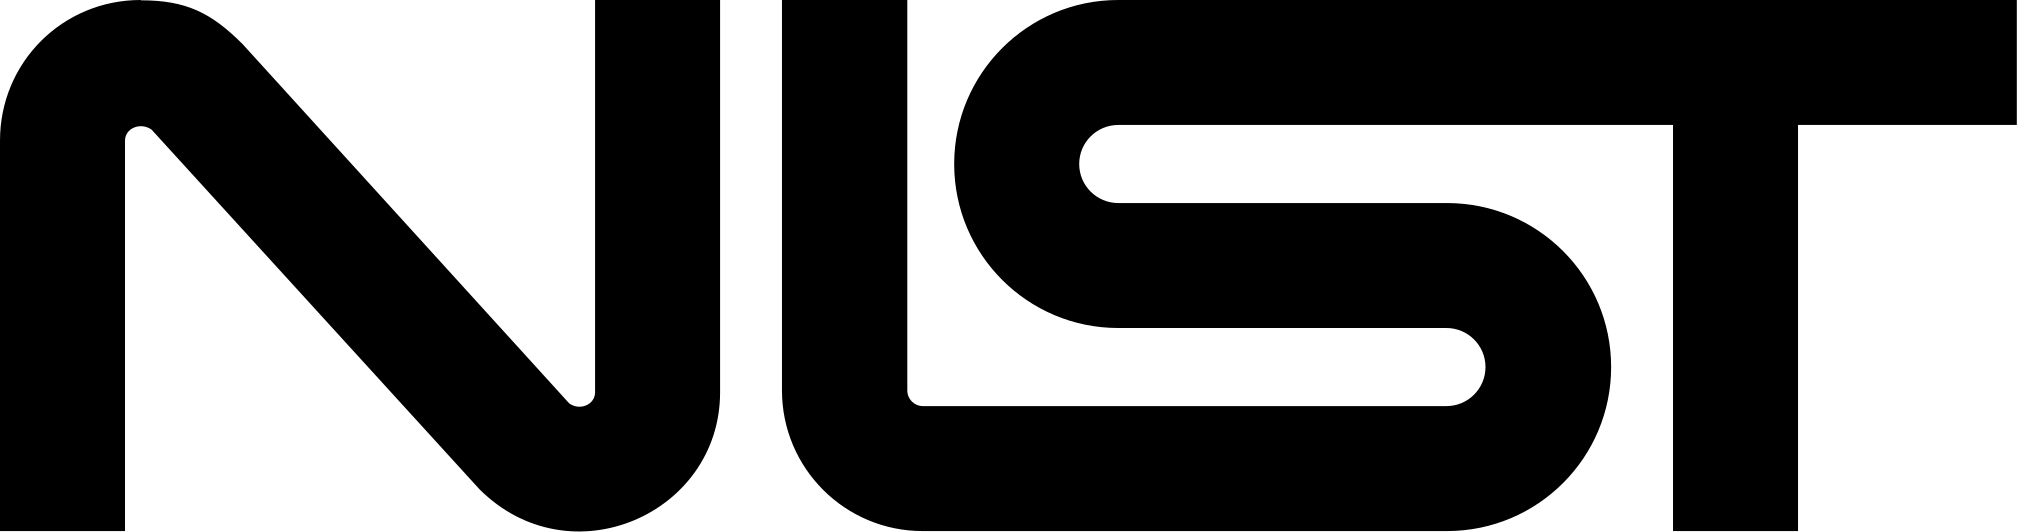
\includegraphics[width=0.9\textwidth]{static/img/NIST.png}
      \end{center}
    \end{column}
  \end{columns}
\end{frame}
    \subsection{Список литературы}
    \begin{frame}{Список литературы}
      \begin{thebibliography}{9}
          \setbeamertemplate{bibliography item}[triangle]
          
          \bibitem{song} 
          Джимми Сонг
          \emph{Python для программирования криптовалют}. 
          О'Рейли, 2020.
          
          \bibitem{PatientZero} 
          PatientZero 
          \emph{Доступно о криптографии на эллиптических кривых}. 
          URL: https://habr.com/ru/articles/335906/
          
          \bibitem{grau} 
          \emph{Визуализация эллиптических кривых в конечном поле}. 
          URL: https://graui.de/code/elliptic2/
        \end{thebibliography}
      \end{frame}
    \subsection{Спасибо за внимание!}
      \begin{frame}
        \centering{Спасибо за внимание!}
      \end{frame}
  \end{document}